%% 
%% Copyright 2026 Elsevier Ltd
%% 
%% This file is part of the 'Elsarticle Bundle'.
%% ---------------------------------------------
%% 
%% It may be distributed under the conditions of the LaTeX Project Public
%% License, either version 1.2 of this license or (at your option) any
%% later version.  The latest version of this license is in
%%    http://www.latex-project.org/lppl.txt
%% and version 1.2 or later is part of all distributions of LaTeX
%% version 1999/12/01 or later.
%% 
%% The list of all files belonging to the 'Elsarticle Bundle' is
%% given in the file `manifest.txt'.
%% 

%% Template article for Elsevier's document class `elsarticle'
%% with numbered style bibliographic references
%% SP 2008/03/01

\documentclass[preprint,12pt, a4paper]{elsarticle}

%% Use the option review to obtain double line spacing
%% \documentclass[authoryear,preprint,review,12pt]{elsarticle}

%% For including figures, graphicx.sty has been loaded in
%% elsarticle.cls. If you prefer to use the old commands
%% please give \usepackage{epsfig}

%% The amssymb package provides various useful mathematical symbols
\usepackage{amssymb}
\usepackage{hyperref}
\usepackage{url}
\setlength{\parindent}{0pt}
\setlength{\parskip}{4pt}
%% The amsthm package provides extended theorem environments
%% \usepackage{amsthm}

%% The lineno packages adds line numbers. Start line numbering with
%% \begin{linenumbers}, end it with \end{linenumbers}. Or switch it on
%% for the whole article with \linenumbers.
%\usepackage{lineno}

\journal{SoftwareX}

\begin{document}
\renewcommand{\labelenumii}{\arabic{enumi}.\arabic{enumii}}

\begin{frontmatter}

\title{pyssms: one Python package for two-dimensional time-to-collision indicators and car-following surrogate safety measures}

\author[affa]{Seyed Saber Naseralavi\corref{cor1}}
\ead{saber\_naseralavi@uk.ac.ir}
\author[affb]{Akram Mazaheri}
\cortext[cor1]{Corresponding author}

\address[affa]{Department of Civil Engineering, Shahid Bahonar University of Kerman, Kerman 7616914111, Iran}
\address[affb]{Department of Civil and Environmental Engineering, Tarbiat Modares University, Tehran 1411944961, Iran}

\begin{abstract}
Surrogate safety measures turn road-user trajectories into numbers that say how close an encounter came to a collision. Two families of them have lived in separate code: two-dimensional indicators defined for any approach angle, and one-dimensional car-following measures built on short motion stories. pyssms is a Python package that puts both on common ground. Time to collision, time advantage, T2 and time gap are read exactly from one convex conflict polygon, and ten car-following measures are implemented from the motion stories they assume. The package reads SSAM, SUMO, VISSIM, LevelX and NGSIM trajectories, smooths them, finds candidate pairs, sorts encounters into a hierarchy, names the faces and corners that touch, and ships 140 conflict windows cut from NGSIM. It depends on NumPy and PyYAML only. Correctness is tested rather than asserted: 143 automated tests, agreement with the printed procedure on 987,695 random encounters, and independent simulations of the motion stories. Applied to 60 highD, 93 exiD and 6 NGSIM freeway recordings, the share of highD rows with a time to collision of 3 s or less is 0.06\,\% if speeds are assumed constant and 26\,\% if the leader is assumed to brake to a stop. All statistics are descriptive. Version 0.1.0 is the initial release of the package.
\end{abstract}

\begin{keyword}
surrogate safety measures \sep time to collision \sep time advantage \sep trajectory data \sep traffic conflicts \sep Python
\end{keyword}

\end{frontmatter}

\section*{Required Metadata}

\section*{Current code version}

\begin{table}[!h]
\begin{tabular}{|l|p{6.5cm}|p{6.5cm}|}
\hline
\textbf{Nr.} & \textbf{Code metadata description} & \textbf{Please fill in this column} \\
\hline
C1 & Current code version & v0.1.0 \\
\hline
C2 & Permanent GitHub link to code/repository used for this code version & \url{https://doi.org/10.5281/zenodo.24050397} \\
\hline
C3 & Legal Code License & BSD 3-Clause License \\
\hline
C4 & Code versioning system used & git \\
\hline
C5 & Software code languages, tools, and services used & Python 3; NumPy, PyYAML; optional: matplotlib \\
\hline
C6 & Compilation requirements, operating environments \& dependencies & Python 3.10 or newer; continuous integration on Linux and Windows with Python 3.10 and 3.13 \\
\hline
C7 & If available Link to developer documentation/manual & \url{https://github.com/sabernaseralavi-60/pyssms/tree/main/docs} \\
\hline
C8 & Support email for questions & saber\_naseralavi@uk.ac.ir \\
\hline
\end{tabular}
\caption{Code metadata (mandatory)}
\label{tab:meta}
\end{table}

\textbf{Main text}\\

\begin{enumerate}

\item \textbf{Motivation and significance}\label{sec:motivation}\\

Ask whether the car-following pairs of a freeway recording are in danger. An analyst who assumes constant speeds flags 0.06\,\% of the sampled highD rows at a time to collision of 3 s or less; one who assumes that the leader brakes to a stop flags 26\,\%. Neither has made an error: each has chosen a motion story. The number in a paper ends a chain of choices, namely a file reader, a smoothing window, a pair filter, a story and a threshold, and the chain is rarely visible. pyssms is built to make it visible.

Surrogate safety measures (SSMs) describe how close road users came to a collision, without waiting for crashes \cite{arun2021,zheng2021}. Drone recordings such as highD, inD, rounD and exiD \cite{krajewski2018,bock2020,krajewski2020,moers2022} and the NGSIM vehicle trajectories \cite{ngsim2017} now supply trajectories at scale, and for years the FHWA Surrogate Safety Assessment Model derived measures from simulated ones \cite{gettman2003}. What is missing is open, tested code that applies the published definitions to such files, so that a number in a paper can be traced to a line of code.

Two traditions need to meet in that code. Laureshyn, Svensson and Hydén \cite{laureshyn2010} defined time to collision (TTC), time advantage (TAdv), T2 and time gap (TG) for any approach angle, with road users represented as rectangles, by enumerating 32 combinations of a corner of one road user and a side of the other. Naseralavi et al. \cite{naseralavi2025} coded ten car-following measures by the short motion story each one assumes: constant speeds, accelerations or jerks for TTC1, TTC2 and TTC3, a braking leader for TTCD, and braking of the follower for DRAC, MDRAC, DCIA, PSD, MPSD and SDI. The first is geometric and works for crossings and merges; the second is kinematic and works along a lane. Each is usually implemented, if at all, on its own and for one data set.

Related open software: Traffic Intelligence \cite{jackson2013,saunier} processes road-safety trajectories and motion predictions, and CommonRoad-CriMe \cite{lin2023} collects criticality measures for automated-vehicle scenarios. For rectangles, vectorised Python code computes the time to collision, the deceleration rate, the proportion of stopping distance, TAdv, a two-dimensional TTC and the anticipated collision time \cite{jiao,jiao2025,venthuruthiyil2022}; the emergency index is published with its authors' code \cite{cheng2025}. In the source read on 2026-11-08, the TAdv of that code takes corner-to-corner intersections of the velocity lines, returns neither T2 nor TG, and comes without file readers or a hierarchy of encounters. A documented search on 2026-11-08 of the Python Package Index, GitHub, Crossref and OpenAlex (log in the repository, docs/lit) found no package that provides TTC, TAdv, T2 and TG of the 2010 paper from one polygon together with the ten car-following measures and the file formats of the common data sets; it is a search, not a systematic review, and the absence of other tools cannot be proved. pyssms is written to close that gap. It (i) reads trajectories, (ii) computes TTC, TAdv, T2 and TG exactly on one conflict polygon, (iii) computes the ten car-following measures, (iv) names the faces and corners that touch, (v) summarises encounters in a hierarchy, and (vi) ships a small bank of conflict windows for tests and teaching. Its numbers are checked against the printed procedure, against simulations and against the data sets' own columns.

\item \textbf{Software description}\label{sec:architecture}\\

\begin{enumerate}
\item \textbf{Software architecture.} pyssms has 19 modules in four layers (read, prepare, compute, report; Fig.~\ref{fig:arch}). Only NumPy and PyYAML are required; matplotlib is optional for plots. The code is typed and documented, and every module states its assumptions in its docstring.

The computing core is one geometric idea. Let $\tau$$_1$ and $\tau$$_2$ be the predicted times at which road users 1 and 2 reach given positions on their paths. The pairs ($\tau$$_1$, $\tau$$_2$) at which the two bodies would overlap form a convex polygon K in the plane of the two predicted arrival times; K is the Minkowski difference of the bodies expressed in that plane (Fig.~\ref{fig:poly}, panel B). Because the bodies are convex and the velocities constant, K is the solution set of a few linear inequalities in ($\tau$$_1$, $\tau$$_2$): eight for two rectangles that move along their length and twelve in general. Undisturbed motion is the diagonal $\tau$$_1$ = $\tau$$_2$. If K meets the diagonal the road users are on a collision course (state A) and TTC is where the diagonal enters K. If K misses it (state B, a crossing course), TAdv is the smallest |$\tau$$_1$ $-$ $\tau$$_2$| over K, and T2 and TG are read from the same polygon as the earliest second arrivals. If K is empty within the horizon there is no overlap (state C). The 32 combinations of the 2010 appendix become one polygon, and parallel paths, standing road users and overlapping bodies need no special case. Path-time diagrams of this kind are classical in robot motion planning \cite{odonnell1989,kant1986}.

Four design rules follow from the opening example. Every assumption (a reaction time, a deceleration, a horizon, a smoothing window) is a named argument; where a default exists it is visible in the signature and the docstring, and the functions of ssm1d take reaction time and decelerations without defaults. A measure that does not exist for a pair is NaN, never zero: TTC is undefined unless the pair is on a collision course. Each module is checked against an independent oracle, such as a time-stepping simulation or an implementation of the printed procedure, and not against itself. Data stay outside the package, which ships only a small NGSIM bank and counts.

\begin{figure}[!htbp]
\centering
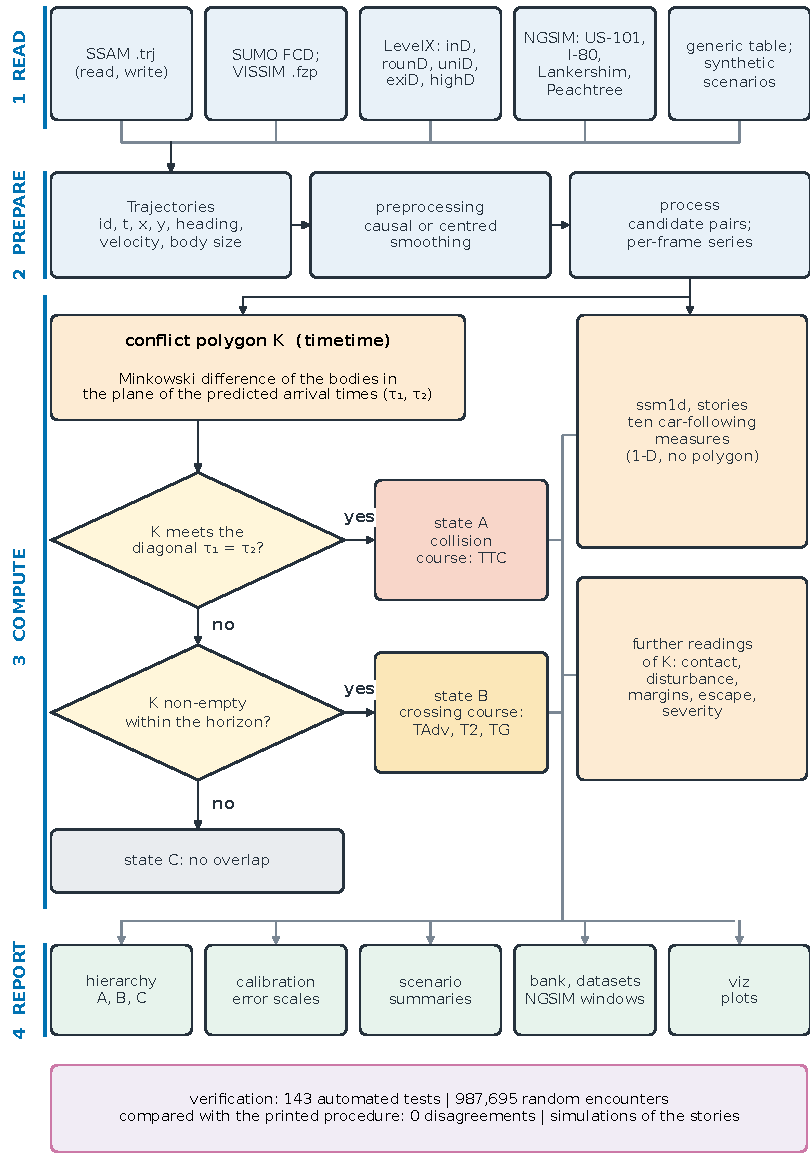
\includegraphics[width=\textwidth]{figures/fig1_architecture.pdf}
\caption{Structure of pyssms: four layers from file readers to reports. The decision sequence sorts every pair and frame into state A, B or C; a second lane takes the leader-follower series to the ten car-following measures, which do not need K. The dashed arrow leads to further readings of the same encounter. The bar at the bottom lists the checks of the package.}
\label{fig:arch}
\end{figure}

\begin{figure}[!htbp]
\centering
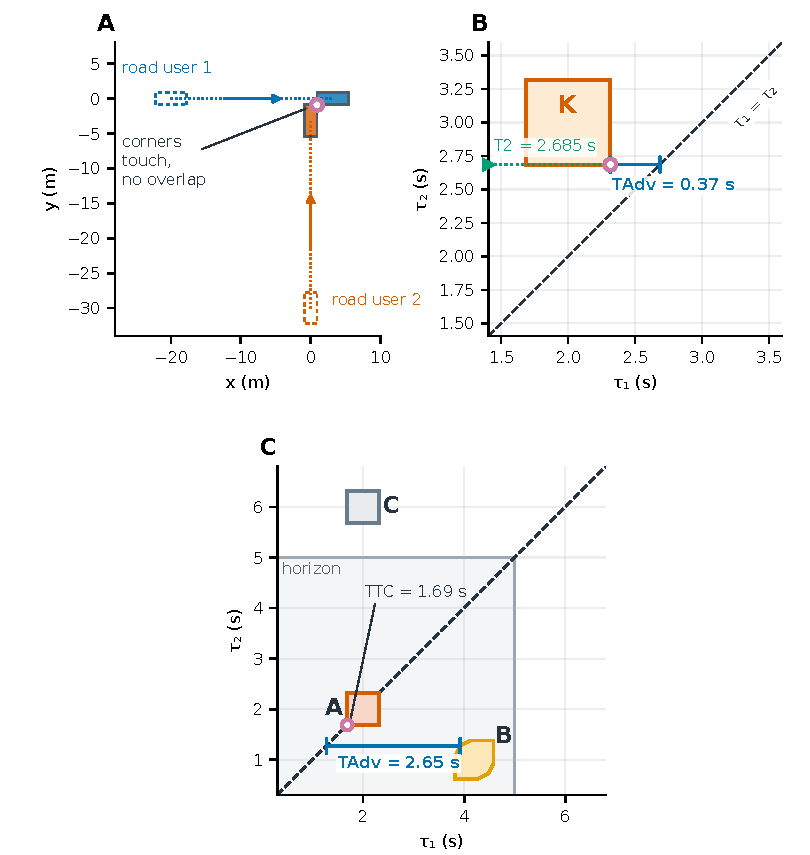
\includegraphics[width=\textwidth]{figures/fig2_polygon.pdf}
\caption{One encounter in three views. (A) Plan view: dashed outlines at the start, filled bodies where they would touch if road user 1 were delayed by TAdv (each body at its own arrival time; circle: touching corners). (B) Conflict polygon K in the plane of the two predicted arrival times, with the diagonal, TAdv and T2. (C) The same construction for three encounters in one plane: the diagonal enters K in state A (TTC), K lies beside the diagonal in state B (TAdv), and K lies outside the horizon (shaded square) in state C.}
\label{fig:poly}
\end{figure}

\item \textbf{Software functionalities.} Readers and preparation. Trajectories are read from SSAM .trj files (reading and writing), SUMO floating-car output, VISSIM .fzp, LevelX files (inD, rounD, uniD, exiD, highD), NGSIM and generic tables into one Trajectories object. The NGSIM reader converts feet to metres and moves the reference from the front centre to the body centre. Causal or centred smoothing is a separate, explicit step.

Indicators. TTC, TAdv, T2 and TG are computed for arrays of encounters, with an 8-row form of the polygon for bodies that move along their length and a general 12-row form for any convex shape. Margins, a smallest-braking search (escape) and a disturbance set add readings of the same polygon. Delta-V and an extended Delta-V \cite{laureshyn2017} and injury-risk curves \cite{lubbe2022} give severity.

Car-following measures. TTC1, TTC2, TTC3, TTCD, DRAC, MDRAC, DCIA, PSD, MPSD and SDI are written from their stories, not copied from printed formulas. Where a printed form differs from its own derivation the differences are listed (docs/ssm1d\_notes.md); reaction time and decelerations are inputs of the functions of ssm1d, without defaults. Table~\ref{tab:ten} lists the measures.

\begin{table}[!ht]
\centering\small
\caption{The ten car-following measures of ssm1d: the motion story each one assumes, its inputs besides the gap and the speeds, its unit, and the direction in which a value is more critical.}\label{tab:ten}
\begin{tabular}{p{1.4cm}p{5.2cm}p{3.5cm}p{1.1cm}p{2.5cm}}
\hline
\textbf{Measure} & \textbf{Motion story} & \textbf{Further inputs} & \textbf{Unit} & \textbf{More critical when} \\
\hline
TTC1 & constant speeds & none & s & smaller \\
TTC2 & constant accelerations & none & s & smaller \\
TTC3 & constant jerks & none & s & smaller \\
TTCD & leader brakes to a stop, follower keeps its speed & leader deceleration & s & smaller \\
DRAC & follower brakes at once to remove the closing speed & none & m/s$^2$ & larger \\
MDRAC & as DRAC after a reaction time & reaction time & m/s$^2$ & larger \\
DCIA & follower keeps its acceleration during the reaction time, then brakes to match speeds at contact & reaction time & m/s$^2$ & larger \\
PSD & gap divided by the follower's stopping distance & follower deceleration & 1 & smaller \\
MPSD & as PSD with the distance covered during the reaction time & follower deceleration, reaction time & 1 & smaller \\
SDI & both brake; 1 if the follower cannot stop behind the stopped leader & both decelerations, reaction time & 0 or 1 & 1 \\
\hline
\end{tabular}
\end{table}

Contact and reporting. The contact module names the face and corner that touch first on a collision course, and the pair that would touch if the road user ahead were delayed by TAdv on a crossing course; the ten corner-side configurations of Jiménez et al. \cite{jimenez2013} come out as classes. Further modules give observed post-encroachment time, a hierarchy of encounters, prediction-error scales, scenario summaries and comparisons, plots, and a bank of conflict windows.

\textbf{Verification.}

The suite has 143 automated tests. The polygon was compared with an independent implementation of the printed 2010 procedure on 1,000,000 random encounters of cars, pedestrians, cyclists and trucks: 987,695 are covered by the procedure (12,305 start with overlapping bodies, which it does not treat), and the two disagree on 0 of the 987,695 for TTC, TAdv, T2, TG and the first road user (Fig.~\ref{fig:verif}). With a side parallel to an axis the printed in-section test needs an exact equality of floating-point numbers; a literal implementation misses the TTC of 6,730 of 49,731 such cases. The car-following measures are tested against independent time-stepping simulations of their stories. The polygon is not faster than a vectorised enumeration of the 32 combinations (4.3 $\mu$s against 4.1 $\mu$s per encounter, a ratio of 1.05); its value is agreement with the printed procedure and one code path for the cases the procedure does not treat (parallel paths, standing road users, overlapping bodies). The general 12-row form, which any convex shape uses, takes 2.18 times as long as the 8-row form.

\begin{figure}[!htbp]
\centering
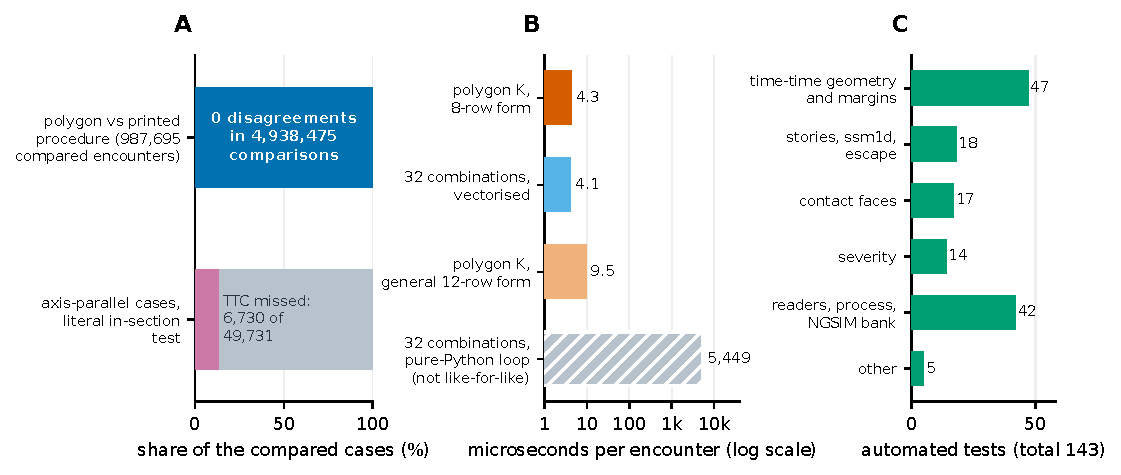
\includegraphics[width=\textwidth]{figures/fig3_verification.pdf}
\caption{Checks of the package. (A) The polygon against the printed procedure: no disagreement in the compared encounters, and the share of axis-parallel cases in which a literal implementation of the procedure misses the TTC. (B) Time per encounter for a million encounters, logarithmic axis; the per-encounter loop is a pure-Python reference and not a like-for-like comparison. (C) Automated tests by area.}
\label{fig:verif}
\end{figure}

\textbf{Usage.}

The listing reads one NGSIM period, smooths it, sorts all encounters into levels, loads the shipped bank, plots one window, and computes the ten car-following measures of a synthetic leader and follower. It ran in about 3 minutes on the first author's computer, most of it in the search of 49,034 encounters of the full period.

\begin{footnotesize}\begin{verbatim}
from pyssms import datasets, hierarchy, io
from pyssms import preprocessing, process, scenario, viz

traj = io.read_ngsim("trajectories-0830am-0845am.txt")
traj = preprocessing.smooth_trajectories(traj, window=5)
enc = process.encounters(traj, horizon=10.0)
print(hierarchy.build_hierarchy(enc).table())

bank = datasets.load_conflict_bank("ngsim")
w = bank.window(bank.select("B")[0])
e = process.pair_series(w, 0, 1)   # TTC, TAdv, T2, TG
viz.plot_indicator_profile(e)

m = scenario.following_measures(   # ten measures, 1-D
    datasets.make("following"), leader=0, follower=1)
\end{verbatim}\end{footnotesize}
\end{enumerate}

\item \textbf{Illustrative examples}\label{sec:examples}\\

\textbf{One encounter, four readings.}

Two cars of 4.5 $\times$ 1.8 m cross at right angles at 10 m/s, 20 m and 30 m from the crossing point (Fig.~\ref{fig:poly}). The polygon K does not meet the diagonal, so the encounter is a crossing course (state B): TAdv is 0.37 s, the horizontal distance from K to the diagonal (panel B), and T2 is 2.685 s. The contact module reports that, were the first road user delayed by TAdv, the two bodies would touch at corners and not overlap (panel A). Panel C puts three encounters in one plane: a collision course (state A) with a TTC of 1.69 s, an oblique crossing (state B) with a TAdv of 2.65 s, and a pair too far apart for the horizon (state C).

\textbf{Ten car-following measures on freeway data.}

We applied the ten measures to follower-leader pairs of 60 highD recordings (30,765,802 pair-frames), 93 exiD recordings (14,968,717) and 6 NGSIM freeway periods (8,238,546), sampled once per second. The leader is the vehicle ahead in the same lane. The reaction time (1 s) and both decelerations (6 m/s$^2$) were fixed before the run; they are assumptions of the stories, not data. No outcome is used, so nothing here ranks a measure or validates it.

The choice of story decides which rows are critical (Fig.~\ref{fig:ten}). On highD 0.06\,\% of sampled rows have TTC1 of 3 s or less but 26.2\,\% have TTCD of 3 s or less, a ratio of 427; on exiD the shares are 0.12\,\% and 32.2\,\%, and on NGSIM 2.4\,\% and 62.7\,\%. TTC1 is defined (finite and within the prediction horizon) for only 3\,\% of highD rows, since it needs a closing pair, and TTCD for 99\,\%. Parameters matter as well, and not always in the same direction: with a reaction time of 1.5 s and decelerations of 4 m/s$^2$, the share of highD rows with TTCD of 3 s or less falls from 26.2\,\% to 11.0\,\%, whereas the share with SDI equal to one rises from 26.2\,\% to 47.7\,\%.

\begin{figure}[!htbp]
\centering
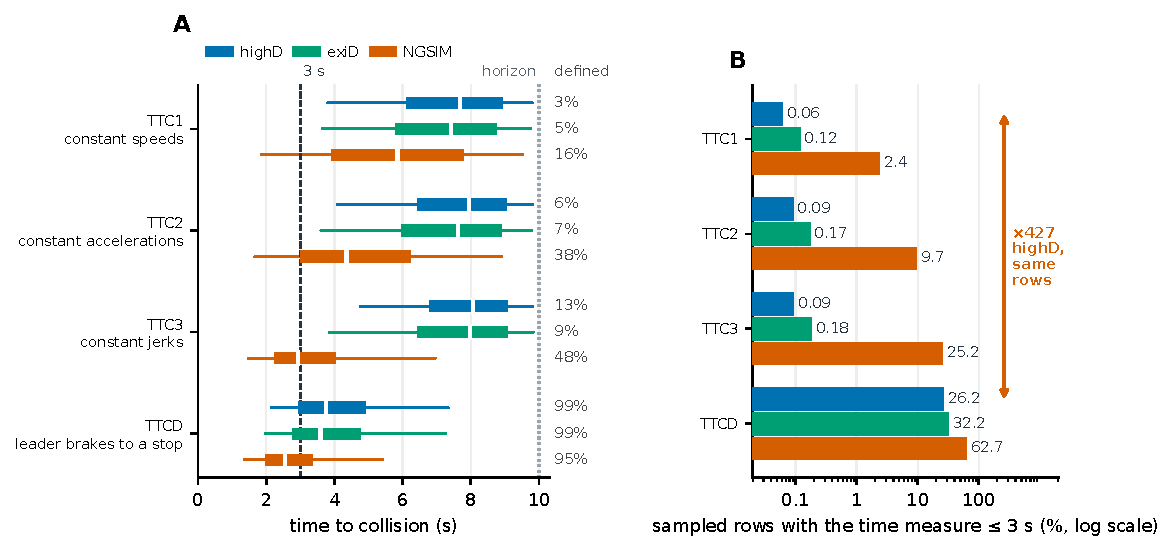
\includegraphics[width=\textwidth]{figures/fig4_ten_measures.pdf}
\caption{The four time measures on three data sets. (A) Range from percentile 5 to percentile 95 (thin line), interquartile range (thick bar) and median (white tick) of the defined values; the percentage is the share of sampled rows where the measure is defined (finite and within the horizon, which cuts off the largest values). (B) Share of sampled rows with the measure at 3 s or less, logarithmic axis; the bracket marks the ratio of TTCD to TTC1 on highD.}
\label{fig:ten}
\end{figure}

The measures also order pairs differently (Fig.~\ref{fig:rho}). MPSD and the polygon's TG rank the pairs alike on all three data sets (Spearman $\rho$ = 0.96, 0.96 and 0.94). TTCD and PSD follow TAdv and TG closely on the German freeways ($\rho$ from 0.86 to 0.92) but less so on NGSIM (TTCD with TAdv 0.80, PSD with TAdv 0.50), whereas TTC1 and TAdv are nearly unrelated on highD ($\rho$ = -0.12). Where both are defined, TTC1 and the polygon TTC rank the pairs identically on highD ($\rho$ = 1.00), but differ in value by up to 1.6 s (highD), 6.4 s (exiD) and 8.4 s (NGSIM), because TTC1 sees only the longitudinal geometry. The polygon TTC exists for 62\,\% of the highD rows where TTC1 is within the horizon; in the other 38\,\% the two bodies miss each other in two dimensions although TTC1 is finite.

\begin{figure}[!htbp]
\centering
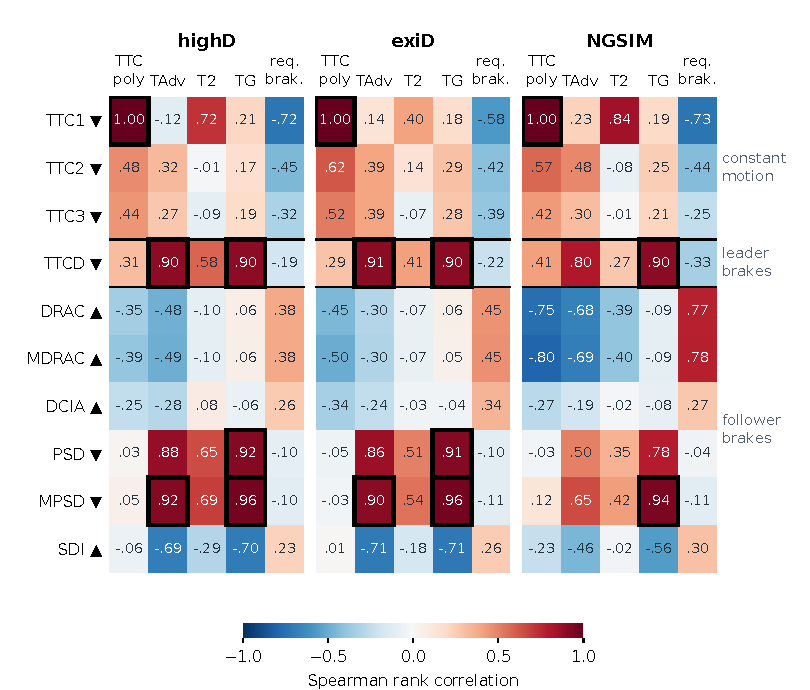
\includegraphics[width=\textwidth]{figures/fig5_correlations.pdf}
\caption{Spearman rank correlation between the ten car-following measures (rows, grouped by motion story; $\blacktriangle$ more critical when larger, $\blacktriangledown$ when smaller) and polygon-based indicators (columns; TTC poly is the polygon TTC), pairwise on defined values. Required braking (req. brak.) is the smallest constant deceleration that avoids a contact within the horizon (module escape). Outlined cells: correlation of 0.90 or more after rounding to two decimals. TTC1 enters only where it exists, and SDI is binary.}
\label{fig:rho}
\end{figure}

Checks guard the reading. On highD the clear gap computed by pyssms equals the data set's own headway within 0.010 m. On exiD the difference lies between -0.09 and 0.05 m from percentile 5 to percentile 95 (largest 2.1 m). On NGSIM it lies between -0.55 and 0.46 m, with a largest value of 109.5 m (lane changes, or the preceding-vehicle column lagging behind the positions); nothing was removed.

\textbf{Hierarchy of encounters and the effect of preprocessing.}

The hierarchy sorts every candidate vehicle pair of a recording into level A (by TTC), B (by TAdv) or C (no overlap), with a split by severity. We ran it on 233 recordings of six data sets (inD, rounD, uniD, exiD, highD and ten NGSIM periods), 4,433,449 candidate pairs of motor vehicles (Fig.~\ref{fig:hier}). The collision-course share runs from 1\,\% of pairs on highD to 36\,\% on NGSIM, and the shape of the hierarchy differs by site: on exiD 30\,\% of pairs are crossing courses against 7\,\% collision courses. The counts are descriptive and say nothing about which encounters were dangerous.

Preprocessing changes the counts. NGSIM's acceleration column differs from the derivative of its speed column by 1.0 m/s$^2$ (US-101) and 4.8 m/s$^2$ (I-80) root mean square, a defect known from the literature \cite{thiemann2008,montanino2015}. At Peachtree Street the share of pairs reaching TTC below 1.5 s is 4.4\,\% on the data set's own positions and speeds and 7.0\,\% after a causal five-frame smoothing (panel B; the two runs differ in positions and in the speed source), and the share of pairs with no overlap falls from 46.0\,\% to 38.4\,\%. The package does not choose for the user: smoothing is a visible step that must be reported.

\begin{figure}[!htbp]
\centering
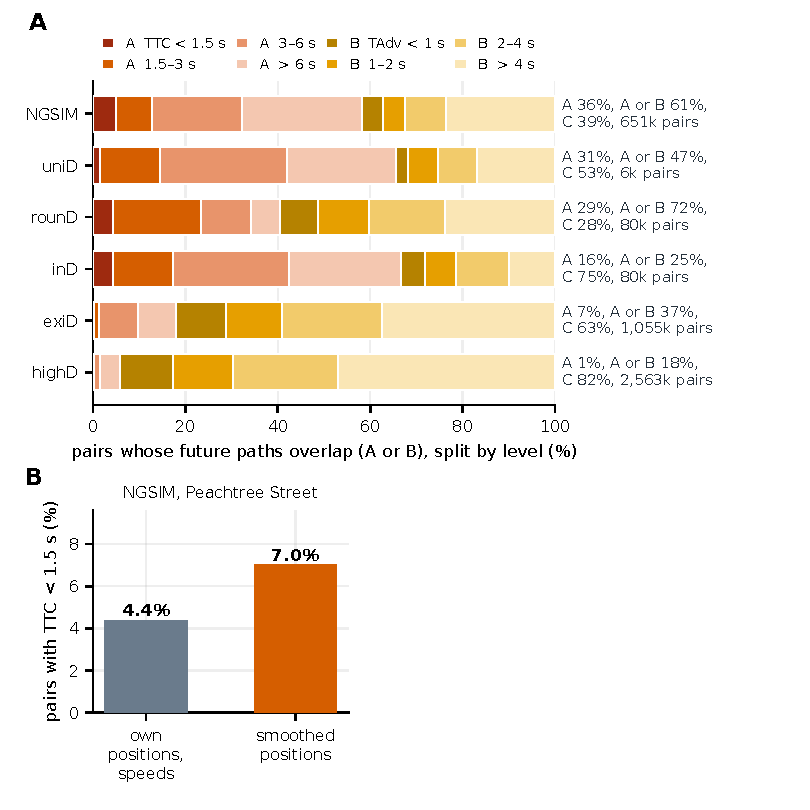
\includegraphics[width=\textwidth]{figures/fig6_hierarchy.pdf}
\caption{(A) Candidate pairs of motor vehicles whose future paths overlap, split into levels A and B (TTC and TAdv classes); the labels give the shares of all pairs in level A and in levels A or B (paths overlap), and the number of pairs. (B) Effect of smoothing on NGSIM, Peachtree Street.}
\label{fig:hier}
\end{figure}

\item \textbf{Impact}\label{sec:impact}\\

What pyssms changes for a researcher is traceability. A safety indicator computed from a drone recording passes through a reader, a preprocessing choice, a pair filter, a motion story and a threshold. In pyssms each is one visible function with stated assumptions, and the numbers in this paper were produced by scripts in the repository from the result files, not typed. The examples show why this matters: the same pairs are critical in 0.06\,\% or 26\,\% of highD rows depending on a story, and an NGSIM count moves with a smoothing window.

The package serves three uses. First, teaching and method comparison: the shipped bank of 140 NGSIM windows (80 chosen by smallest TTC, 40 by smallest TAdv, 20 by smallest distance; 0.7 MB) lets a student run every indicator without downloading a data set. The windows are chosen by the package's own indicators, so they are test material, not a sample of traffic: in the 80 windows chosen by smallest TTC the smallest TTC has a median of 0.014 s and never exceeds 0.14 s, at centre distances of 2.3 to 7.7 m, so the rectangular bodies are about to touch. Second, wherever the 2010 indicators are needed for arbitrary convex shapes, one tested function replaces hand-coded enumeration of corner and side combinations. Third, a common platform on which the validation of indicators against outcomes can be done: a reader, an outcome extractor (braking onset), and counts of encounters per level are in place. Such a validation was named the most critical next step of the car-following framework \cite{naseralavi2025}; evasive-action onset is a candidate outcome \cite{johnsson2022}. It has not been done here, and the examples above must not be read as one.

The software is young. Version 0.1.0 is the initial release of the package; it has no record of use outside the authors' own work and no citations yet, and it is installed with pip from the Python Package Index or from its repository. The shipped NGSIM windows carry the licence text of the Federal Highway Administration (a modified Creative Commons Attribution 2.0 licence); nothing from the LevelX data sets is shipped except counts and prediction-error scales. The limits that matter for use are the assumptions of the model. K assumes constant velocity and translation without rotation, so a turning vehicle is predicted along its current heading; the ten car-following measures are one-dimensional and need a leader and a follower along a lane; their parameters are assumptions; and no two-dimensional version of those ten measures exists yet. A companion methods manuscript on the geometry of K is in preparation. The package does not replace criticality metrics designed for automated driving \cite{westhofen2023}; it supplies the indicators of the 2010 and 2025 papers with tests.

\item \textbf{Conclusions}\label{sec:conclusions}\\

pyssms brings the two-dimensional indicators of the 2010 framework and the ten car-following measures of the 2025 framework into one tested Python package that reads the files of the common data sets. Verification is part of the package: 143 tests, agreement with the printed procedure on 987,695 encounters, and simulations of the motion stories. The examples show that results depend on choices that code makes visible: the motion story, its parameters and the smoothing of positions. Everything reported is descriptive. The next steps are validation against observed outcomes and a two-dimensional version of the car-following measures.

\end{enumerate}

\section*{Acknowledgements}

The authors thank the providers of the highD, inD, rounD, exiD and NGSIM data for making them available for research.

\section*{Declaration of generative AI and AI-assisted technologies in the manuscript preparation process}

During the preparation of this work the authors used Claude (Anthropic) for study planning, code and analysis scripts, figures, literature screening, and drafting and editing of the text. The authors reviewed, verified and edited the output and take full responsibility for the content of the publication.

\section*{CRediT authorship contribution statement}

Seyed Saber Naseralavi: Conceptualization, Methodology, Software, Validation, Formal analysis, Investigation, Data curation, Writing – original draft, Writing – review \& editing, Visualization. Akram Mazaheri: Validation, Investigation, Data curation, Writing – review \& editing.

\section*{Funding}

This research did not receive any specific grant from funding agencies in the public, commercial, or not-for-profit sectors.

\section*{Declaration of competing interest}

The authors declare that they have no known competing financial interests or personal relationships that could have appeared to influence the work reported in this paper.

\section*{Data availability}

The code is available at https://github.com/sabernaseralavi-60/pyssms (BSD 3-Clause licence), and version 0.1.0 is archived on Zenodo \cite{pyssms_zenodo}. The shipped NGSIM windows come from the Federal Highway Administration NGSIM data under a modified Creative Commons Attribution 2.0 licence (credit FHWA and NGSIM). The LevelX data sets are available from their providers on request; only aggregated counts are shipped. The numbers of this paper are reproduced by paper\_softwarex/make\_numbers.py.

\begin{thebibliography}{00}

\bibitem{arun2021} Arun A, Haque MM, Washington S, Sayed T, Mannering F. A systematic review of traffic conflict-based safety measures with a focus on application context. Anal Methods Accid Res 2021;32:100185. \url{https://doi.org/10.1016/j.amar.2021.100185}.

\bibitem{zheng2021} Zheng L, Sayed T, Mannering F. Modeling traffic conflicts for use in road safety analysis: a review of analytic methods and future directions. Anal Methods Accid Res 2021;29:100142. \url{https://doi.org/10.1016/j.amar.2020.100142}.

\bibitem{krajewski2018} Krajewski R, Bock J, Kloeker L, Eckstein L. The highD dataset: a drone dataset of naturalistic vehicle trajectories on German highways for validation of highly automated driving systems. In: 2018 21st International Conference on Intelligent Transportation Systems (ITSC); 2018. p. 2118--25. \url{https://doi.org/10.1109/ITSC.2018.8569552}.

\bibitem{bock2020} Bock J, Krajewski R, Moers T, Runde S, Vater L, Eckstein L. The inD dataset: a drone dataset of naturalistic road user trajectories at German intersections. In: 2020 IEEE Intelligent Vehicles Symposium (IV); 2020. p. 1929--34. \url{https://doi.org/10.1109/IV47402.2020.9304839}.

\bibitem{krajewski2020} Krajewski R, Moers T, Bock J, Vater L, Eckstein L. The rounD dataset: a drone dataset of road user trajectories at roundabouts in Germany. In: 2020 IEEE 23rd International Conference on Intelligent Transportation Systems (ITSC); 2020. p. 1--6. \url{https://doi.org/10.1109/ITSC45102.2020.9294728}.

\bibitem{moers2022} Moers T, Vater L, Krajewski R, Bock J, Zlocki A, Eckstein L. The exiD dataset: a real-world trajectory dataset of highly interactive highway scenarios in Germany. In: 2022 IEEE Intelligent Vehicles Symposium (IV); 2022. p. 958--64. \url{https://doi.org/10.1109/IV51971.2022.9827305}.

\bibitem{ngsim2017} U.S. Department of Transportation, Federal Highway Administration. Next Generation Simulation (NGSIM) vehicle trajectories and supporting data [dataset]; 2017. \url{https://doi.org/10.21949/1504477}.

\bibitem{gettman2003} Gettman D, Head L. Surrogate safety measures from traffic simulation models. Transp Res Rec 2003;1840:104--15. \url{https://doi.org/10.3141/1840-12}.

\bibitem{laureshyn2010} Laureshyn A, Svensson Å, Hydén C. Evaluation of traffic safety, based on micro-level behavioural data: theoretical framework and first implementation. Accid Anal Prev 2010;42:1637--46. \url{https://doi.org/10.1016/j.aap.2010.03.021}.

\bibitem{naseralavi2025} Naseralavi S, Soltanirad M, Ranjbar E, Jimee K, Lucero M, Baghersad M, et al. A short-term storytelling framework for understanding surrogate safety measures in intelligent vehicle interactions. Future Transp 2025;5:86. \url{https://doi.org/10.3390/futuretransp5030086}.

\bibitem{jackson2013} Jackson S, Miranda-Moreno LF, St-Aubin P, Saunier N. Flexible, mobile video camera system and open source video analysis software for road safety and behavioral analysis. Transp Res Rec 2013;2365:90--8. \url{https://doi.org/10.3141/2365-12}.

\bibitem{saunier} Saunier N. Traffic Intelligence: tools for transportation data processing [software], MIT licence. Python Package Index. \url{https://pypi.org/project/trafficintelligence/} (accessed 2026-11-07).

\bibitem{lin2023} Lin Y, Althoff M. CommonRoad-CriMe: a toolbox for criticality measures of autonomous vehicles. In: 2023 IEEE Intelligent Vehicles Symposium (IV); 2023. p. 1--8. \url{https://doi.org/10.1109/IV55152.2023.10186673}.

\bibitem{jiao} Jiao Y. Two-Dimensional-Time-To-Collision [software], MIT licence. GitHub. \url{https://github.com/Yiru-Jiao/Two-Dimensional-Time-To-Collision} (accessed 2026-11-07).

\bibitem{jiao2025} Jiao Y. Vectorised surrogate safety measures for traffic interactions in two-dimensional space [software], MIT licence. GitHub; 2025. \url{https://github.com/Yiru-Jiao/SSMsOnPlane} (accessed 2026-11-08).

\bibitem{venthuruthiyil2022} Venthuruthiyil SP, Chunchu M. Anticipated collision time (ACT): a two-dimensional surrogate safety indicator for trajectory-based proactive safety assessment. Transp Res Part C 2022;139:103655. \url{https://doi.org/10.1016/j.trc.2022.103655}.

\bibitem{cheng2025} Cheng H, Jiang Y, Zhang H, Chen K, Huang H, Xu S, et al. Emergency index (EI): a two-dimensional surrogate safety measure considering vehicles' interaction depth. Transp Res Part C 2025;171:104981. \url{https://doi.org/10.1016/j.trc.2024.104981}.

\bibitem{odonnell1989} O'Donnell PA, Lozano-Pérez T. Deadlock-free and collision-free coordination of two robot manipulators. In: Proceedings, 1989 International Conference on Robotics and Automation; 1989. p. 484--9. \url{https://doi.org/10.1109/robot.1989.100033}.

\bibitem{kant1986} Kant K, Zucker SW. Toward efficient trajectory planning: the path-velocity decomposition. Int J Robot Res 1986;5:72--89. \url{https://doi.org/10.1177/027836498600500304}.

\bibitem{laureshyn2017} Laureshyn A, De Ceunynck T, Karlsson C, Svensson Å, Daniels S. In search of the severity dimension of traffic events: extended Delta-V as a traffic conflict indicator. Accid Anal Prev 2017;98:46--56. \url{https://doi.org/10.1016/j.aap.2016.09.026}.

\bibitem{lubbe2022} Lubbe N, Wu Y, Jeppsson H. Safe speeds: fatality and injury risks of pedestrians, cyclists, motorcyclists, and car drivers impacting the front of another passenger car as a function of closing speed and age. Traffic Saf Res 2022;2:000006. \url{https://doi.org/10.55329/vfma7555}.

\bibitem{jimenez2013} Jiménez F, Naranjo JE, García F. An improved method to calculate the time-to-collision of two vehicles. Int J Intell Transp Syst Res 2013;11:34--42. \url{https://doi.org/10.1007/s13177-012-0054-4}.

\bibitem{thiemann2008} Thiemann C, Treiber M, Kesting A. Estimating acceleration and lane-changing dynamics from Next Generation Simulation trajectory data. Transp Res Rec 2008;2088:90--101. \url{https://doi.org/10.3141/2088-10}.

\bibitem{montanino2015} Montanino M, Punzo V. Trajectory data reconstruction and simulation-based validation against macroscopic traffic patterns. Transp Res Part B 2015;80:82--106. \url{https://doi.org/10.1016/j.trb.2015.06.010}.

\bibitem{johnsson2022} Johnsson C, Laureshyn A. Identification of evasive manoeuvres in traffic interactions and conflicts. Traffic Saf Res 2022;3:000012. \url{https://doi.org/10.55329/erqd8683}.

\bibitem{westhofen2023} Westhofen L, Neurohr C, Koopmann T, Butz M, Schütt B, Utesch F, et al. Criticality metrics for automated driving: a review and suitability analysis of the state of the art. Arch Comput Methods Eng 2023;30:1--35. \url{https://doi.org/10.1007/s11831-022-09788-7}.

\bibitem{pyssms_zenodo} Naseralavi SS, Mazaheri A. pyssms: surrogate safety indicators for road-user encounters on a time-time conflict polygon [software]. Version 0.1.0. Zenodo; 2026. \url{https://doi.org/10.5281/zenodo.24050397}.

\end{thebibliography}

\section*{Current executable software version}

v0.1.0, installed with pip install pyssms==0.1.0 or from the repository (\url{https://github.com/sabernaseralavi-60/pyssms}).

\end{document}
